\documentclass[10pt,a4paper]{article}
\usepackage[utf8]{inputenc} % para poder usar tildes en archivos UTF-8
%\usepackage[spanish]{babel} % para que comandos como \today den el resultado en castellano
%\usepackage{a4wide} % márgenes un poco más anchos que lo usual
\usepackage[conEntregas]{caratula}

% Para que el código de JavaScript se vea bonito
\usepackage{color}
\definecolor{lightgray}{rgb}{.9,.9,.9}
\definecolor{darkgray}{rgb}{.4,.4,.4}
\definecolor{purple}{rgb}{0.65, 0.12, 0.82}
\usepackage{listings}
\lstdefinelanguage{JavaScript}{
  keywords={typeof, new, true, false, catch, function, return, null, catch, switch, var, if, in, while, do, else, case, break},
  keywordstyle=\color{blue}\bfseries,
  ndkeywords={class, export, boolean, throw, implements, import, this},
  ndkeywordstyle=\color{darkgray}\bfseries,
  identifierstyle=\color{black},
  sensitive=false,
  comment=[l]{//},
  morecomment=[s]{/*}{*/},
  commentstyle=\color{purple}\ttfamily,
  stringstyle=\color{red}\ttfamily,
  morestring=[b]',
  morestring=[b]"
}
\lstset{
   language=JavaScript,
   backgroundcolor=\color{lightgray},
   extendedchars=true,
   basicstyle=\footnotesize\ttfamily,
   showstringspaces=false,
   showspaces=false,
   numbers=left,
   numberstyle=\footnotesize,
   numbersep=9pt,
   tabsize=2,
   breaklines=true,
   showtabs=false,
   captionpos=b
}

%hyperlinks
\usepackage{hyperref}

% achicar los margenes
\addtolength{\oddsidemargin}{-.875in}
\addtolength{\evensidemargin}{-.875in}
\addtolength{\textwidth}{1.75in}
\addtolength{\topmargin}{-.875in}
\addtolength{\textheight}{1.75in}

\begin{document}

\titulo{Base de datos noSQL}
\subtitulo{Trabajo Práctico 2}

\materia{Base de datos}

\integrante{Guillamon, Gonzalo}{97/12}{gonzaguillamon@gmail.com}
\integrante{Toffoletti, Luis}{827/11}{luis.toffoletti@gmail.com}
\integrante{Zanollo, Florencia}{934/11}{florenciazanollo@gmail.com}
% Pongan cuantos integrantes quieran

\maketitle

%\tableofcontents <--completar índice?

\newpage
\section{Introducción}
  En este trabajo práctico se presenta un ejemplo de trabajo con bases de datos noSQL (a partir de una base de datos relacional),
asi como el uso de la técnica de sharding para lograr que los datos se almacenen de forma distribuida y la técnica de map reduce,
que se utiliza para realizar consultas eficientes basadas en computo paralelo utilizada en bases de datos distribuidas.
El sistem de bases de datos a utilizar es MongoDB. MongoDB es un sistema de bases de datos orientado a documentos, guardando
la estructura de los datos en documentos tipo JSON (javascript object notation) que se almacenan en colecciones. Si estuvieramos
en el modelo relacional, cada colección tendría como una tabla y cada registro sería un documento.\\
  La estructura a utilizar para los documentos es la siguiente:
\begin{itemize}

\item 
  Facturas: En las facturas se desea almacenar, para el usuario que corresponde, nombre completo y número de id
  para poder identificarlo, la fecha para diferenciar a que mes corresponde cada factura y el detalle pertinente a cada cliente.
  Esto es, qué publicaciones realizé mediante el pago de un abono fijo (y en que monto consiste dicho abono) y las ventas que 
  realizó a comisión.
  \begin{lstlisting}[language=JavaScript]
  Facturas
  {
      usuario: {id, nombre, apellido},
      fecha: fecha
      abonoFijo: { publicaciones: [titulos], abono },
      comisiones: [ { publicacion: {titulo}, comision a pagar } ]
  }
  \end{lstlisting}
\item 
  Ventas: En este documento se extrae un resumen de los datos relacionados a una venta. Los datos que nos interesan son
  el id de la publicación, quién vendió, quién compró, que calificación se asignaron mutuamente, de cuánto fue el importe de la venta
  y que comisión corresponde cobrarle al vendedor por dicha venta.
  \begin{lstlisting}[language=JavaScript]
  Ventas:
  {
      publicacionId: id,
      importe: total de la venta,
      vendedor: {id vendedor, nombre},
      comprador: {id comprador, nombre},
      calificacionVendedor: calificacion vendedor,
      calificacionComprador: calificacion comprador,
      comision: porcentaje de comsion cobrada por la venta
  }
  \end{lstlisting}
\item 
  Publicaciones: Este documento es un resumen de cada publicación, que únicamente indica si una publicación pertenece a un servicio o a un articulo,
  el título de dicha publicación y su número de identificación.
  \begin{lstlisting}[language=JavaScript]
  Publicaciones
  {
      Id: id,
      Tìtulo: titulo,
      Tipo de publicación: servicio/articulo
  }
  \end{lstlisting}

\end{itemize}

La estructura de los documentos está definida según lo especificado en la base de datos relacional implementada en el trabajo práctico anterior,
asi como su correpondiente modelo conceptual. Los documentos contienen la información necesaria para realizar las consultas Map-Reduce
detalladas mas adelante.\\

\newpage
\section{Consultas SQL}
Para generar los documentos, se debería extraer la información de la base de datos relacional generada en el trabajo práctico.
A continuación se detallan las consultas en lenguaje SQL necesarias:

  \begin{lstlisting}[language=SQL]
/*Consulta para obtener los datos para emitir la factura mensual de un usuario*/

Select		publicacionId,
		titulo,
		sum(precioPorUnidad * cantidadDeUnidades * comision) as comision
From publicaciones as p 
Join compraventa as cv on p.publicacionId= cv.publicacionId 
Join articulos as a on a.publicacionId=p.publicacionID
Join tipoPublicacion as tp on tp.idTipoPublicacion=p.tipo 
Where cv.fecha.month() >= now.month()-1 
And idTipoPublicacion= 1|2|3 
And p.email= {usuario al que corresponde la factura} 
Group by PublicaciónId, Título

#Solo para las que son oro o plata, las ruby de oriente tienen un abono fijo

  \end{lstlisting}
  \begin{description}
 \item[linea 5] Únicamente para las publicaciones oro y plata.
 \item[linea 10] Obtenemos sólo las publicaciones correspondientes al último mes.
 \item[linea 11] 1= Rubí, 2= Oro, 3= Plata
 \item[linea 12] El email (que es la clave primaria del usuario) se reemplaza por un id en los documentos.
 \item[Nota Adicional] El monto fijo a abonar por las publicaciones rubi de oriente se puede consultar aparte, ya que
 no se usa en la consulta (a diferencia de la comision)
  \end{description}

\newpage
\section{Map Reduce}
MapReduce es un modelo de programación para el procesamiento y creación de grandes colecciones de datos.

Consiste de dos partes:
\begin{itemize}
 \item Map() se encarga de filtrar y organizar los datos, produciendo una lista de pares (clave, valor) por cada llamada. Luego de esto el framework agrupa los pares con la misma clave, creando un grupo por cada una de las diferentes claves generadas.
 \item Reduce(clave, valores) aplica funciones sobre los valores agrupados en el map. Por ejemplo, suma todos los valores, saca el promedio, etc. Retornando un resultado por cada clave.
\end{itemize}

Notar que estos procedimientos (Map y Reduce) son paralelizables, con lo cual pueden ser distribuidos en diferentes unidades (por ejemplo clusters) para su procesamiento.

A continuación listamos todas las consultas a implementar, utilizando MapReduce, requeridas, con su respectivo código y una pequeña explicación del mismo.

\subsection{El importe total de ventas por usuario}

\begin{lstlisting}[language=JavaScript]
var mapFunctionA = function(){
	emit(this.vendedor, this.importe)
};

var reduceFunctionA = function(userId, importes){
	return Array.sum(importes);
}

db.Ventas.mapReduce( mapFunctionA, reduceFunctionA, {out: "mapReduceA"} )

db.mapReduceA.find()
\end{lstlisting}

\begin{description}
 \item[linea 9] Se aplica el MapReduce sobre la colección Ventas.
 \item[linea 2] Como clave se eligió el id del usuario que realiza la venta (i.e. el e-mail del vendedor) y el valor es el importe de la misma.
 \item[linea 5] Con esto se obtiene una lista por vendedor con todos los importes de sus compras.
 \item[linea 6] Los cuales son sumados y se retorna dicha suma.
\end{description}

\newpage
%-----------------------------------------------------------------------------------------------
\subsection{La reputación historica de cada usuario según la calificación}

\begin{lstlisting}[language=JavaScript]
var mapFunctionB = function(){
	emit(this.vendedor, this.calificacionVendedor);
	emit(this.comprador, this.calificacionComprador);
};

var reduceFunctionB = function(userId, calificaciones){
	suma = Array.sum(calificaciones);
	promedio = suma / calificaciones.length
	return promedio;
}

db.Ventas.mapReduce( mapFunctionB, reduceFunctionB, {out: "mapReduceB"} )

db.mapReduceB.find()
\end{lstlisting}

\begin{description}
 \item[linea 12] Se aplica el MapReduce sobre la colección Ventas.
 \item[lineas 2 y 3] Se emiten dos datos, uno que contiene el id del vendedor y otro del comprador, ambos con la calificación correspondiente como valor.
 \item[linea 6] Con esto se obtiene una lista por usuario con todas sus calificaciones (tanto de compras como de ventas).
 \item[lineas 7 y 8] Se retorna el promedio de las calificaciones (por cada usuario).
\end{description}

%-----------------------------------------------------------------------------------------------
\subsection{Las operaciones con comisión más alta}

\begin{lstlisting}[language=JavaScript]
404 NOT FOUND
\end{lstlisting}

\newpage
%-----------------------------------------------------------------------------------------------
\subsection{El monto total facturado por año}

\begin{lstlisting}[language=JavaScript]
var mapFunctionD = function(){
	facturaciones = new Array();

	if(this.hasOwnProperty('abonoFijo')){
		var abono = this.abonoFijo.abono;
		facturaciones.push(abono);
	}

	if(this.hasOwnProperty('comisiones')){
		var comisiones = this.comisiones;

		for (var i = 0; i < comisiones.length; i++) {
			facturaciones.push(comisiones[i].comision)
		}
	}

	emit(this.fecha.slice(this.fecha.length-2, this.fecha.length), facturaciones)
};

var reduceFunctionD = function(year, facturaciones){
	
	facturacionesFlattened = facturaciones.reduce(function(a, b){return a.concat(b)}, []);

	facturacionAnual = Array.sum(facturacionesFlattened);

	return facturacionAnual;
}

db.Facturas.mapReduce( mapFunctionD, reduceFunctionD, {out: "mapReduceD"} )

db.mapReduceD.find()
\end{lstlisting}

\begin{description}
 \item[linea 29] Se aplica el MapReduce sobre la colección Facturas.
 \item[lineas 4 a 7] Si el usuario tiene facturación por abono fijo (i.e. Rubí Oriente) se agrega dicha facturación a la lista de facturaciones.
 \item[lineas 9 a 15] Si el usuario tiene una o más facturaciones por comisión se agregan todas ellas a la lista de facturaciones.
 \item[linea 17] Se utiliza como clave el año.
 \item[linea 20] Con esto se obtiene una lista por año con todas las facturaciones (de comisiones o abonos, de todos los usuarios).
 \item[lineas 24 y 26] Se suman todas las facturaciones y se retorna dicha suma.
\end{description}

\newpage
%-----------------------------------------------------------------------------------------------
\subsection{El monto total facturado por año de las operaciones pertenecientes a usuarios con suscripciones Rubí Oriente}

\begin{lstlisting}[language=JavaScript]
var mapFunctionE = function(){
	facturaciones = new Array();

	if(this.hasOwnProperty('abonoFijo')){
		var abono = this.abonoFijo.abono;
		facturaciones.push(abono);
	
		if(this.hasOwnProperty('comisiones')){
			var comisiones = this.comisiones;

			for (var i = 0; i < comisiones.length; i++) {
				facturaciones.push(comisiones[i].comision)
			}
		}

		emit(this.fecha.slice(this.fecha.length-2, this.fecha.length), facturaciones)
	}
};

var reduceFunctionE = function(year, facturaciones){
	
	var facturacionesFlattened = 0;
	facturacionesFlattened = facturaciones.reduce(function(a, b){return a.concat(b)}, []);

	facturacionAnual = Array.sum(facturacionesFlattened);
	return (facturacionAnual);
}

db.Facturas.mapReduce( mapFunctionE, reduceFunctionE, {out: "mapReduceE"} )

db.mapReduceE.find()
\end{lstlisting}

La funcionalidad es igual al anterior pero en este caso sólo se emiten todas las facturaciones si el usuario posee un abono fijo (i.e. Rubí Oriente).\\

\newpage
%-----------------------------------------------------------------------------------------------
\subsection{El total de las publicaciones por tipo de publicación (productos, servicios, mixtas}

\begin{lstlisting}[language=JavaScript]
var mapFunctionF = function(){
	emit(this.tipoDePublicacion, this.id);
};

var reduceFunctionF = function(tipoDePublicacion, publicaciones){
	return publicaciones.length;
}

db.Publicaciones.mapReduce( mapFunctionF, reduceFunctionF, {out: "mapReduceF"} )

db.mapReduceF.find()
\end{lstlisting}

\begin{description}
 \item[linea 9] Se aplica el MapReduce sobre la colección Publicaciones.
 \item[linea 2] Se toma el tipo de publicación como clave, el valor es el id (único para cada publicación).
 \item[linea 5] Con esto se obtiene una lista de todas las publicaciones agrupadas por tipo de publicación.
 \item[linea 6] Se retorna la cantidad de publicaciones en cada grupo.
\end{description}
\newpage
\section{Sharding}
\subsection{Introducción}

Sharding es la solución que utiliza MongoDB para brindar un acceso a la información almacenada en un tiempo razonable
a medida que aumenta el volumen de datos. 
Permite escalar horizontalmente, es decir agregar nuevas computadoras para distribuir la información.
A continuación describimos a grandes rasgos el funcionamiento de este sistema, se evita entrar en ciertos detalles
específicos de los algoritmos y procesos involucrados porque no resulta fundamental para entender la solución propuesta.\\

\subsection{Estructura de un sharded cluster}

Una colección es dividida en subconjuntos denominados "shards" (se debe configurar un campo del esquema como `shard key'), cada shard
contiene chunks que poseen información en un rango del shard key configurado, de esta manera la información con una shard key similar
se mantendrá próxima (en la mayoría de los casos). 

\begin{figure}[h!]
 \centering
 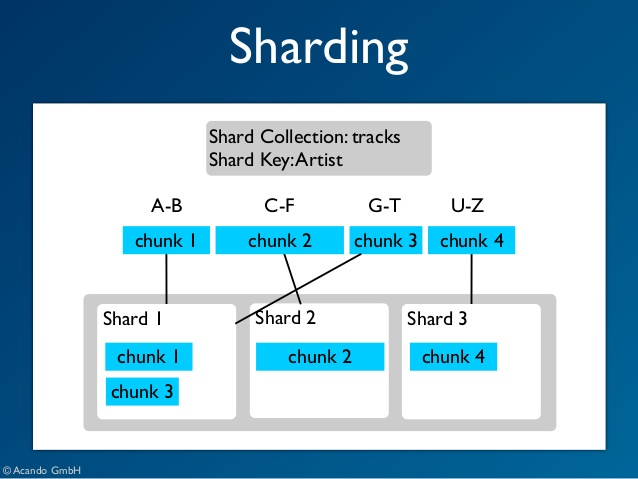
\includegraphics[scale=0.35,keepaspectratio=true]{./sharding.jpg}
 % sharding.jpg: 638x479 pixel, 72dpi, 22.51x16.90 cm, bb=0 0 638 479
 \caption{Diagrama de sharding}
\end{figure}

Por ejemplo, si en una colección se elige `mes del año' como `shard key', y tengo tres
chunks, para el primer rango puedo tener los datos de Enero a Abril, para el segundo de Abril a Agosto, y el último de Agosto a Diciembre.
A medida que se agregue información, puede suceder que se dividan estos chunks, y quede por ejemplo un chunk por mes del año.
A partir de ese momento no será posible dividir para formar nuevos rangos, por lo tanto los chunks se vuelven cada vez más grandes.

\begin{figure}[h!]
 \centering
 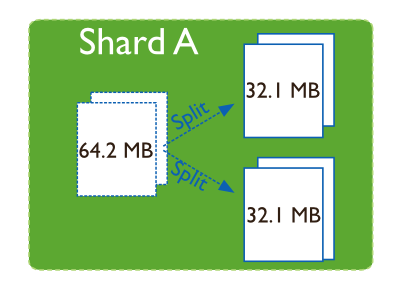
\includegraphics[scale=0.5,keepaspectratio=true]{./split-chunk.png}
 % split-chunk.png: 400x288 pixel, 72dpi, 14.11x10.16 cm, bb=0 0 400 288
 \caption{Division de chunk}
\end{figure}

\subsection{Balanceo y migración}

Los shards se distribuirán en diferentes servidores, lo deseable es contar con la información distribuida de la mejor forma
posible para optimizar las lecturas y escrituras. Además de dividirse, un chunk puede ser migrado de un shard a otro, de 
esta forma se busca balancear la carga entre los servidores.

\begin{figure}[h!]
 \centering
 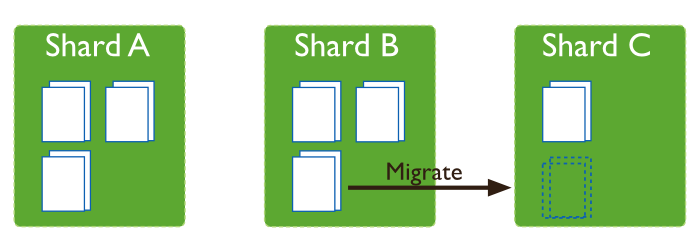
\includegraphics[scale=1,keepaspectratio=true]{./sharding-migrating.png}
 % sharding-migrating.png: 700x252 pixel, 126dpi, 14.11x5.08 cm, bb=0 0 400 144
 \caption{Migración de chunk}
\end{figure}


\subsection{Elección de `Shard key'}

A partir de lo desarrollado, podemos concluir que si queremos utilizar sharding en nuestra colección, resulta fundamental
escoger una `shard key' apropiada.
No hay manera de elegir una clave perfecta, para eso se tienen en cuenta una serie de criterios sobre como se comportan los
datos que manejamos.\\

\begin{itemize}
\item 
Cardinalidad: que tanto puede dividirse el rango de valores, lo deseable es tener una cardinalidad alta, es decir que pueda
generar gran cantidad de rangos. Un ejemplo de alta cardinalidad sería el DNI, de baja puede ser el código de provincia (en
última instancia siempre hay que tener en cuenta el contexto en el que se usan los datos).
\item 
Distribución de las escrituras: lo ideal es distribuir las escrituras de manera uniforme entre los shards, si se escoge una
clave que crece de manera monótona, resulta en un exceso de inserts sobre un único shard.
\item 
Distribución de las lecturas: como en el caso de las escrituras, queremos obtener distribución uniforme.
\item 
Tipo de consultas: tener en cuenta que consultas se realizarán sobre la colección, si involucra búsqueda por rango o un documento
en particular, en cualquier caso lo deseable es que se accedan la menor cantidad de shards posibles. Para eso es necesario
que la shard key esté presente en la consulta efectuada. Por ejemplo si quiero consultar documentos por mes, puedo configurar
una 'shard key' compuesta por mes y algún otro campo, de esta forma la información de un mes en particular estará almacenada en un mismo shard
(de vuelta depende del caso, pero en general sucedería así).\end{itemize}


\subsection{Implementación}

Se utiliza la arquitectura de prueba
\begin{figure}[h!]
 \centering
 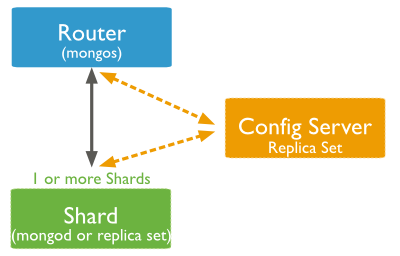
\includegraphics[scale=0.5,keepaspectratio=true]{./sharded-cluster-test-architecture.png}
 % sharded-cluster-test-architecture.png: 400x256 pixel, 72dpi, 14.11x9.03 cm, bb=0 0 400 256
 \caption{Test Architecture}
\end{figure}

Trabajando sobre publicaciones con el siguiente esquema.

\begin{lstlisting}[language=JavaScript]
	{
	"id": (Integer),
	"titulo": (String),
	"tipoDePublicacion": (productos | servicios | mixta),
	"fecha": (Date)
	}
\end{lstlisting}

Generamos los datos de forma aleatoria(uniformemente) sobre un período de años acotado (5 años), `tipo de publicación' puede tomar tres valores
(servicios, productos y mixta).\\

Observaciones:
\begin{itemize}
\item En los siguientes gráficos, el eje x representa el número de iteración de ingreso de datos, en cada una se insertan 20000 documentos.
\item Se decidió representar algunos de los gráficos con barras ya que había mucha colisión entre las lineas, creemos que esta reprensetación ayuda visualmente.
\end{itemize}


Realizamos la experimentación para tres formas de sharding distintas:

\subsubsection{Shard por índice simple: Tipo de publicación}
En primera instancia escogimos `tipo de publicación' como shard key. Obtuvimos una distribución pareja, ya que eran 3 shards
para 3 rangos posibles. A simple vista podría parecer una buena clave, pero hay que tener en cuenta que los datos reales
podrían tener otra distribución, y la baja cardinalidad en ese caso sería un problema, suponiendo un 90\% de publicaciones de artículos 
implicaría tener los shards totalmente desbalanceados.

\begin{figure}[h!]
 \centering
 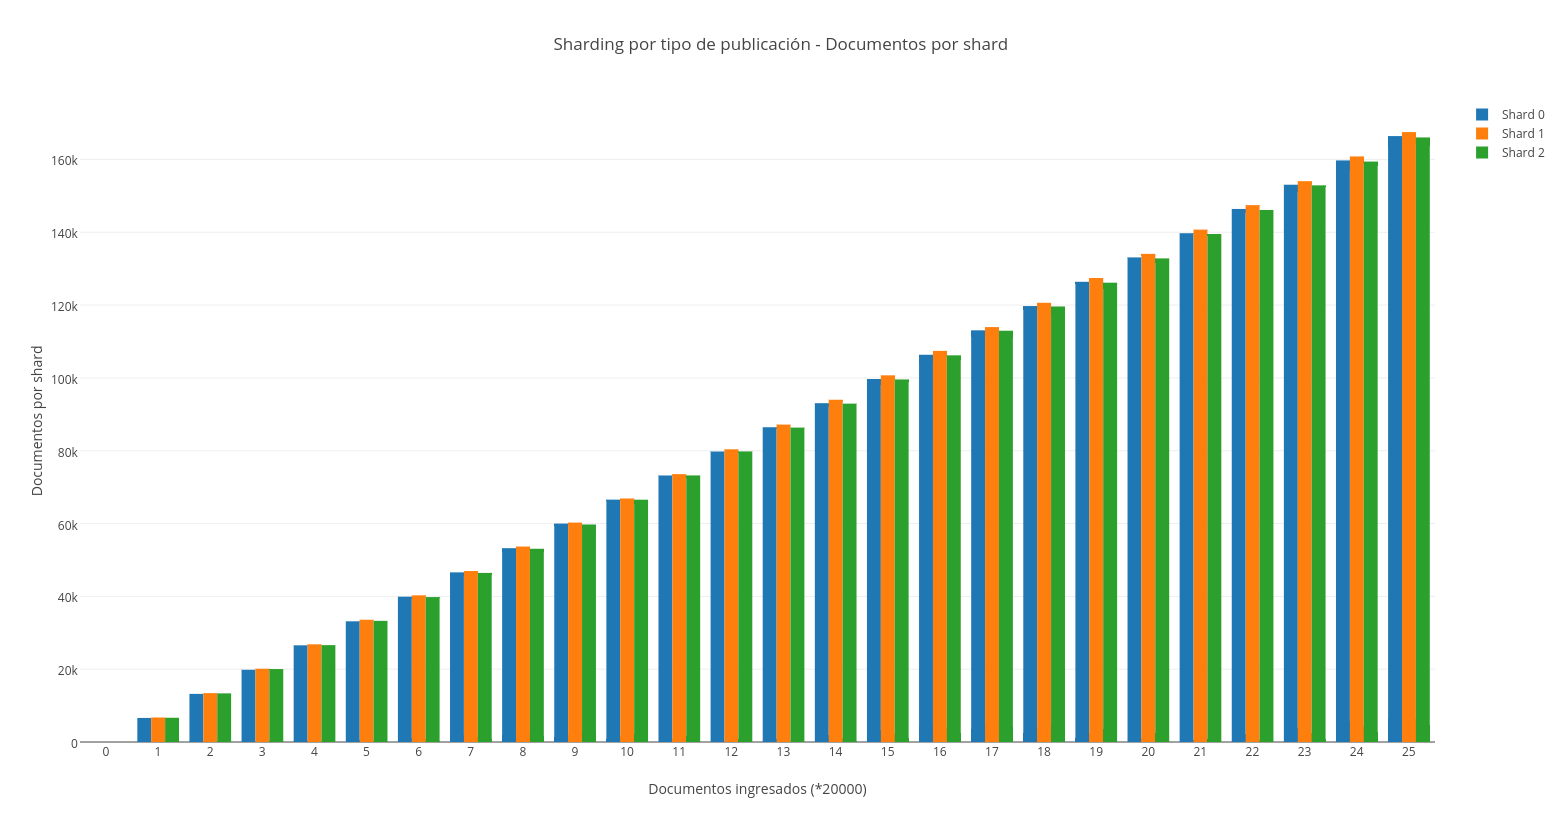
\includegraphics[scale=0.3,keepaspectratio=true]{./ShardingPorTipoDePublicacion-DocumentosPorShard.png}
 \caption{Documentos por Shard}
\end{figure}
 
Con los datos obtenidos a través de las pruebas, generamos gráficos a partir de otros parámetros como datos estimados por chunk y datos por shard, los omitimos en el
informe porque no agregan información interesante.

Para observar mejor el gráfico se puede acceder mediante el siguiente link a su representación online:
\begin{itemize}
 \item \href{https://plot.ly/~fzanollo/13/sharding-por-tipo-de-publicacion-documentos-por-shard/}{Documentos por shard}
\end{itemize}

\newpage
\subsubsection{Shard por índice simple: Fecha}
Analizando los resultados obtenidos en el punto anterior, nos dimos cuenta que esa clave presentaba muchos inconvenientes y
decidimos utilizar otro índice simple, en este caso la fecha, que resultó más interesante. A medida que se insertaron los 
datos se puede observar como se produce el balanceo de shards a través de la división y migración de los chunks, ya que es una clave con 
cardinalidad alta. Hay que tener en cuenta que los datos fueron generados de forma aleatoria, quizás en un caso real las fechas serían 
consecutivas lo que deriva en que las inserciones apunten al mismo shard.

\begin{figure}[h!]
 \centering
 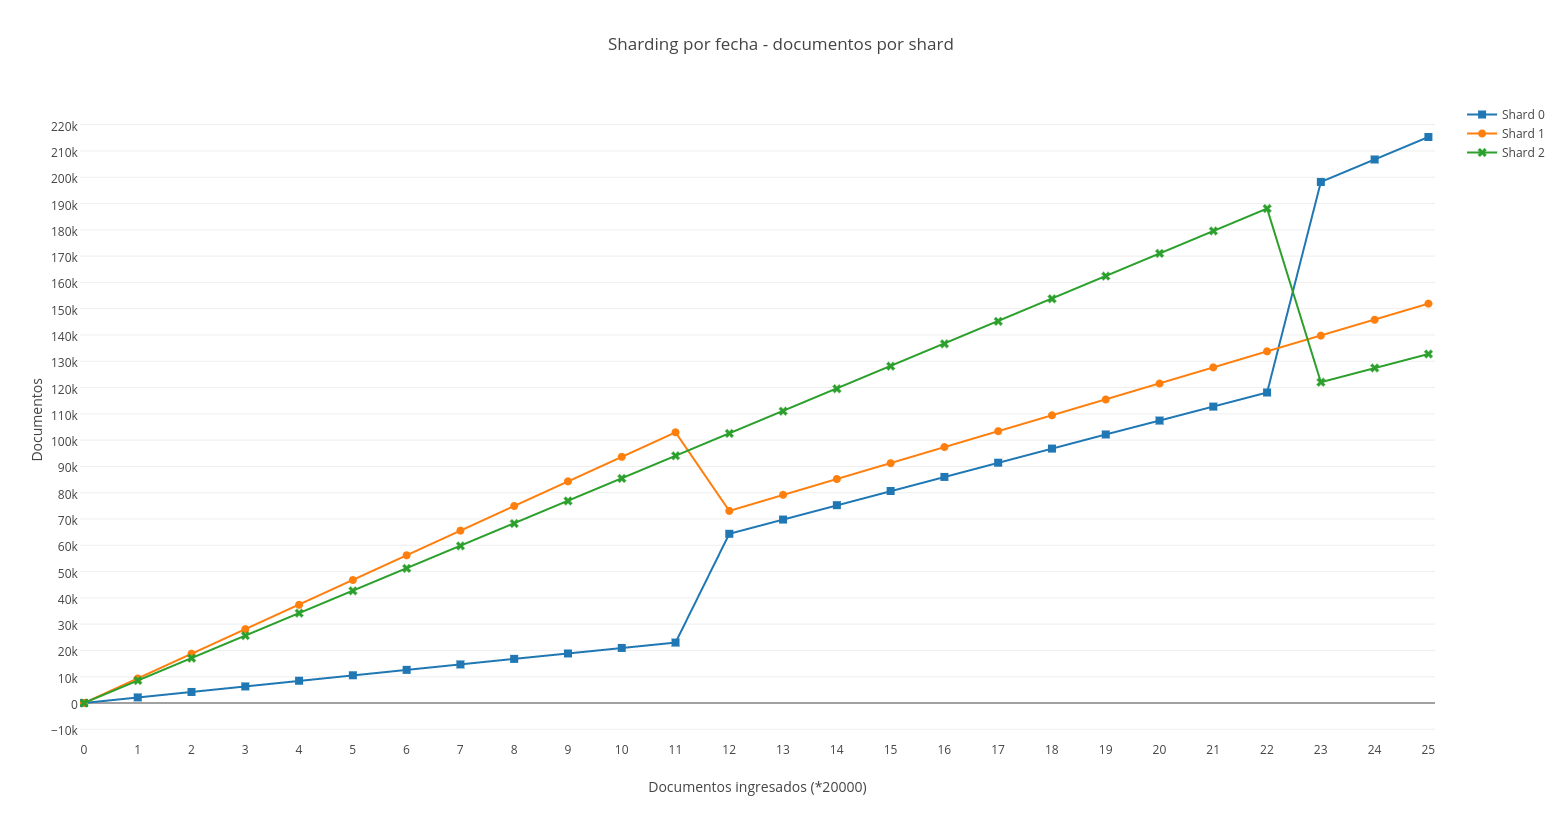
\includegraphics[scale=0.3,keepaspectratio=true]{./fecha-documentos-por-shard.png}
 \caption{Documentos por shard}
\end{figure}

Aquí se observa como se distribuye la carga de datos por shard, no es una distribución perfectamente uniforme pero crecen en general al mismo ritmo. Los cambios bruscos
se deben a migraciones de datos, posiblemente por un chunk muy grande que fue dividido y luego una parte migrada a otro shard.

\begin{figure}[h!]
 \centering
 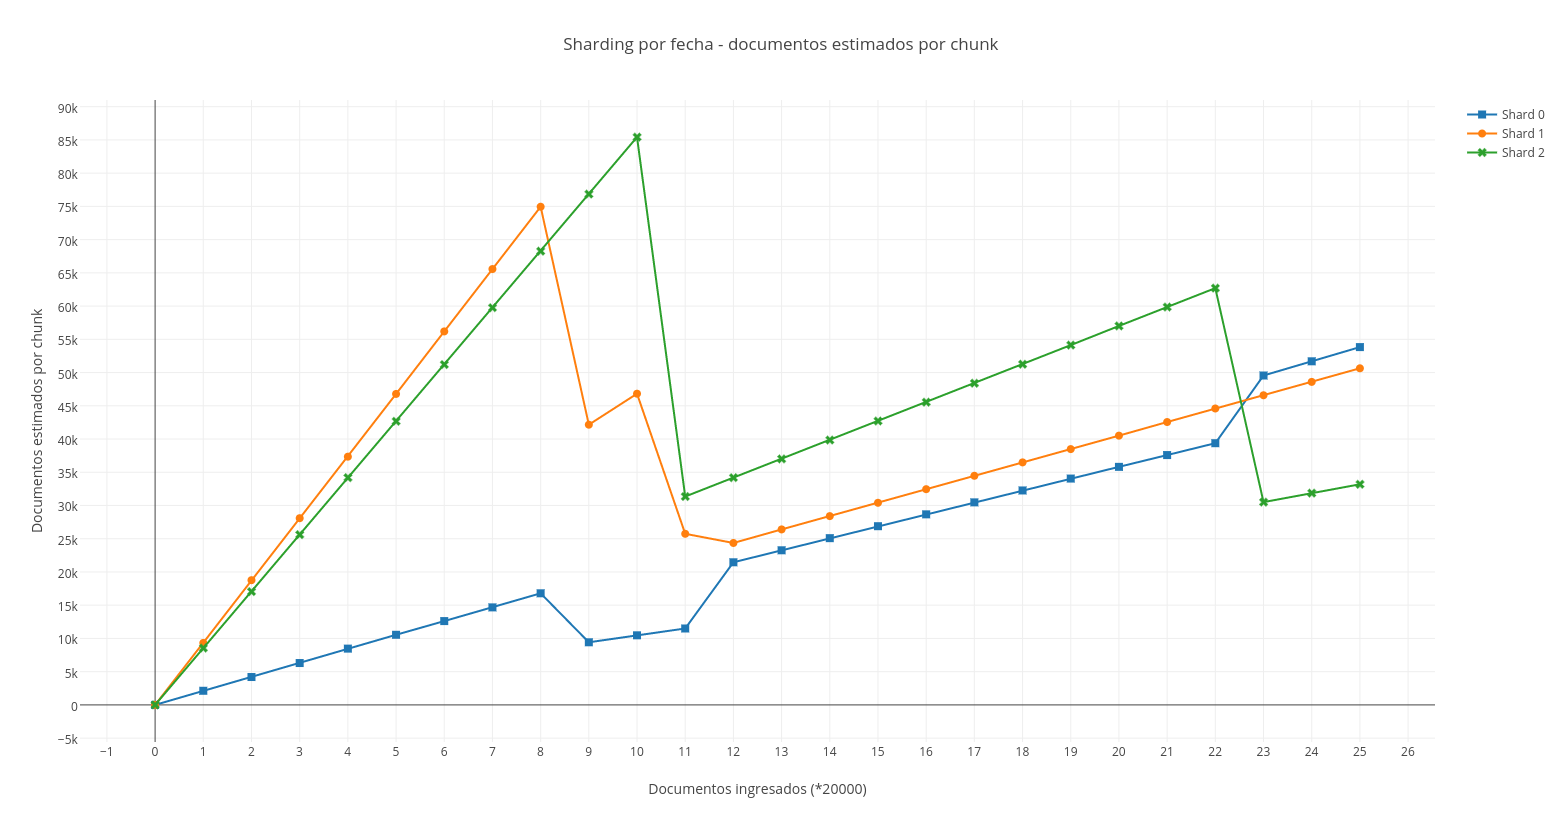
\includegraphics[scale=0.3,keepaspectratio=true]{./fecha-documentos-estimados-por-chunk.png}
 \caption{Datos por chunk}
\end{figure}

En la figura se observa la evolución del promedio de datos por chunk para cada shard, las primeras iteraciones presentan muchas fluctuaciones, debido a las divisiones y migraciones
de chunks, luego se observa como se estabiliza y se mantiene esa tendencia.

\begin{figure}[h!]
 \centering
 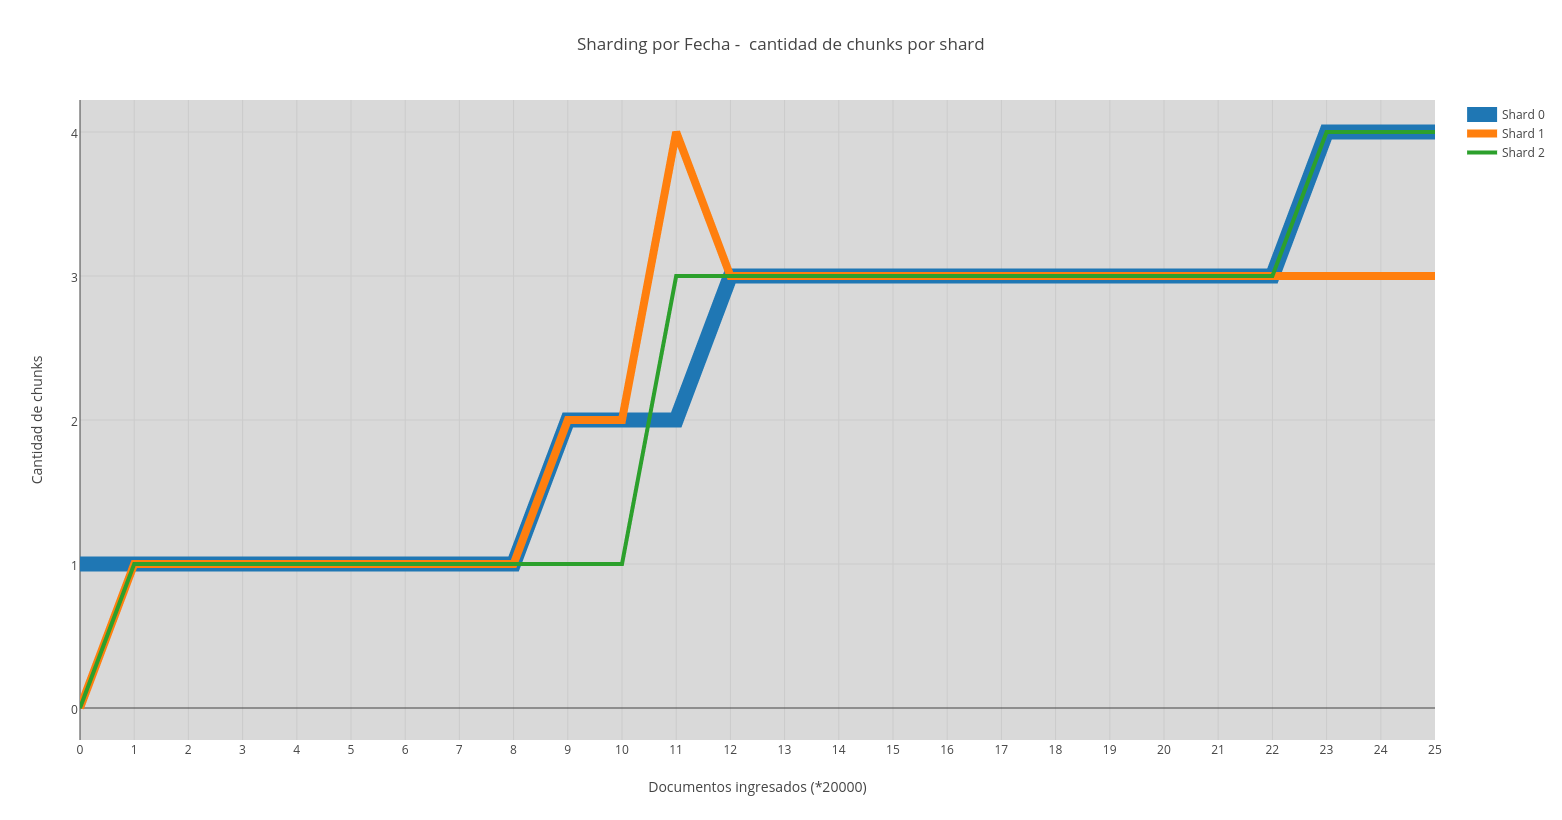
\includegraphics[scale=0.3,keepaspectratio=true]{./Fecha-cantidad-de-chunks-por-shard.png}
 \caption{Chunks por shard}
\end{figure}

Por último se muestra la cantidad de chunks por shard, permitiendo comparar mejor los gráficos anteriores.\\

Para observar mejor los gráficos se pueden acceder mediante los siguientes links a su representación online:
\begin{itemize}
 \item \href{https://plot.ly/~fzanollo/22/sharding-por-fecha-documentos-por-shard/}{Documentos por shard}
 \item \href{https://plot.ly/~fzanollo/31/sharding-por-fecha-documentos-estimados-por-chunk/}{Documentos estimados por chunk}
 \item \href{https://plot.ly/~fzanollo/47/sharding-por-fecha-cantidad-de-chunks-por-shard/}{Cantidad de chunks por shard}
\end{itemize}

\newpage
\subsubsection{Shard por Hash: Id}
Por último se utiliza un índice hash sobre el campo `id' que genera Mongo a cada documento. Se eligió este campo ya que, al no poder elegir una clave compuesta, todos los campos generados por nosotros para las versiones de prueba se repetían demasiado (lo que hubiese generado hash parecidos, sino iguales).

\begin{figure}[h!]
 \centering
 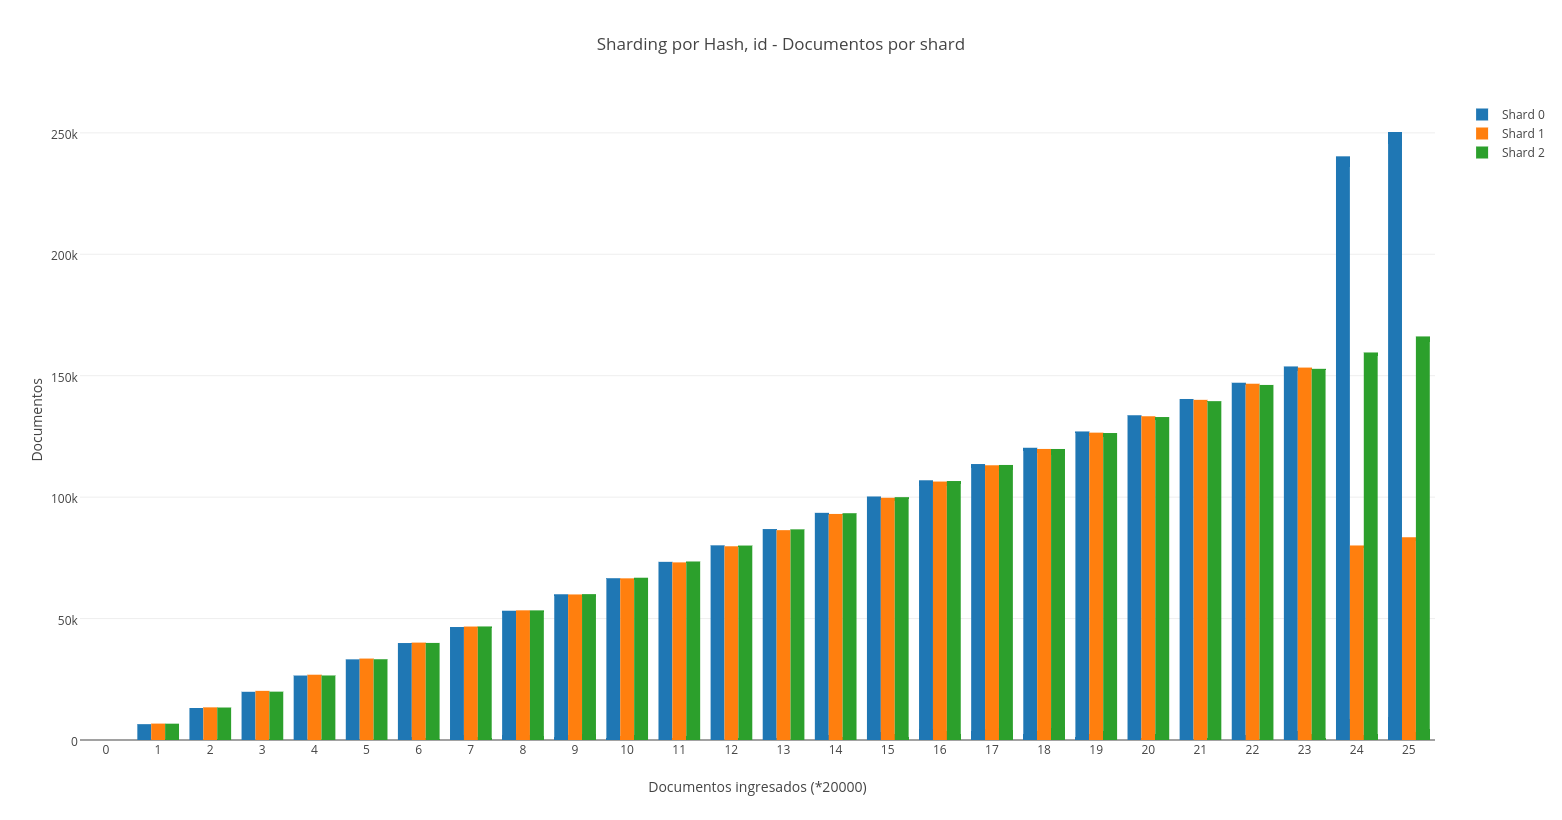
\includegraphics[scale=0.3]{./hash-documentos-por-shard.png}
 \caption{Documentos por shard}
\end{figure}

Vemos como se distribuyen uniformemente a medida que se ingresan datos. El cambio que se observa en la iteración 24 se puede deber a una mala elección de migración, esto, a medida que los datos crecen, se va corrigiendo. Ya que se espera, de un buen algoritmo de hash, una distribución uniforme.

\begin{figure}[h!]
 \centering
 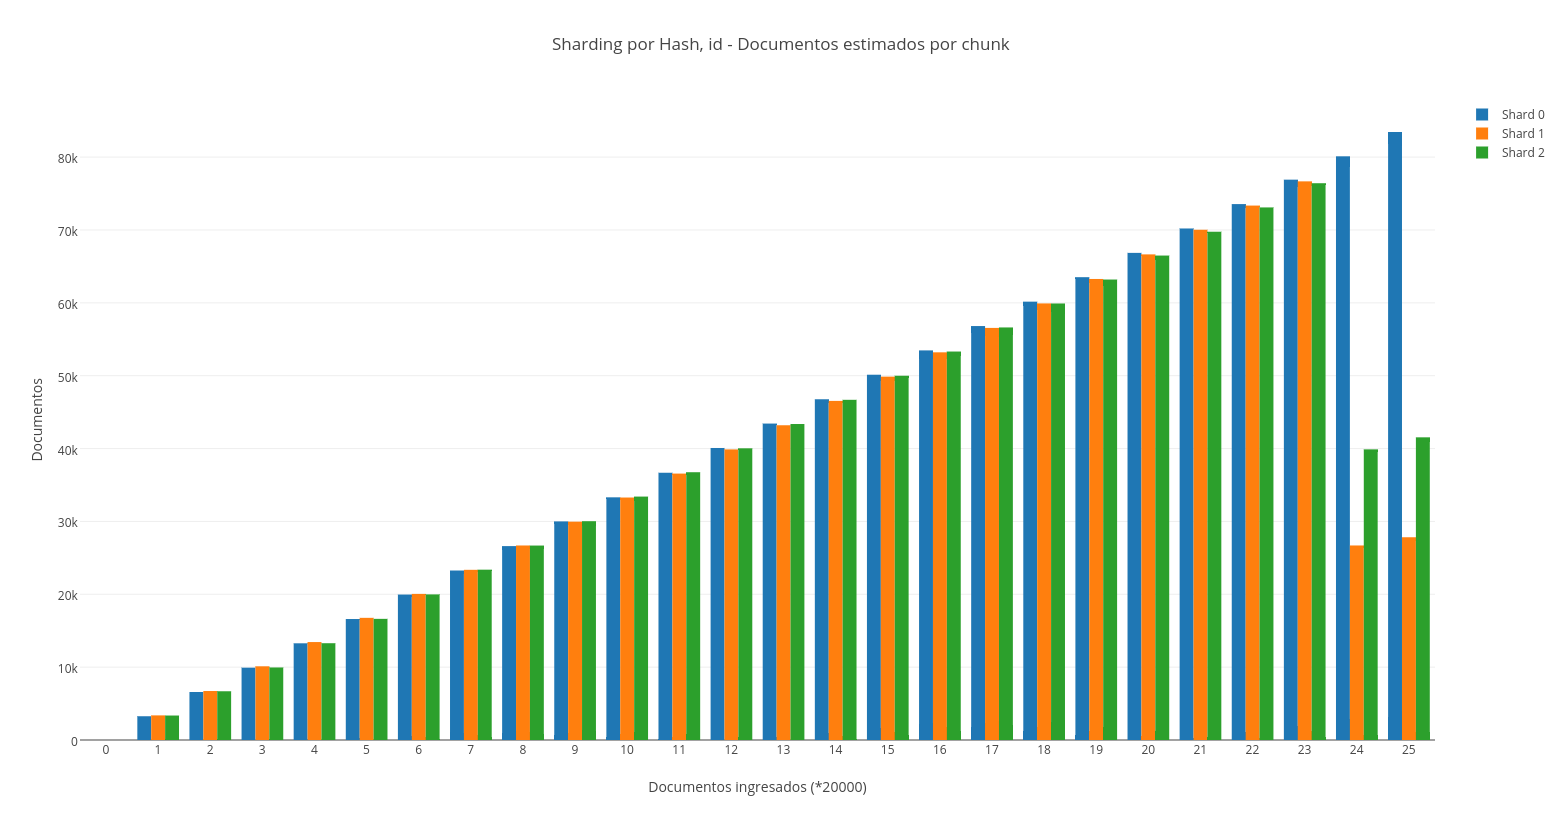
\includegraphics[scale=0.3]{./hash-documentos-estimados-por-chunk.png}
 \caption{Datos por chunk}
\end{figure}

Se observa que los chunks quedan desbalanceados en la iteración nro 24.
Quedando más cantidad de datos por chunk en el shard 0.\\

\begin{figure}[h!]
 \centering
 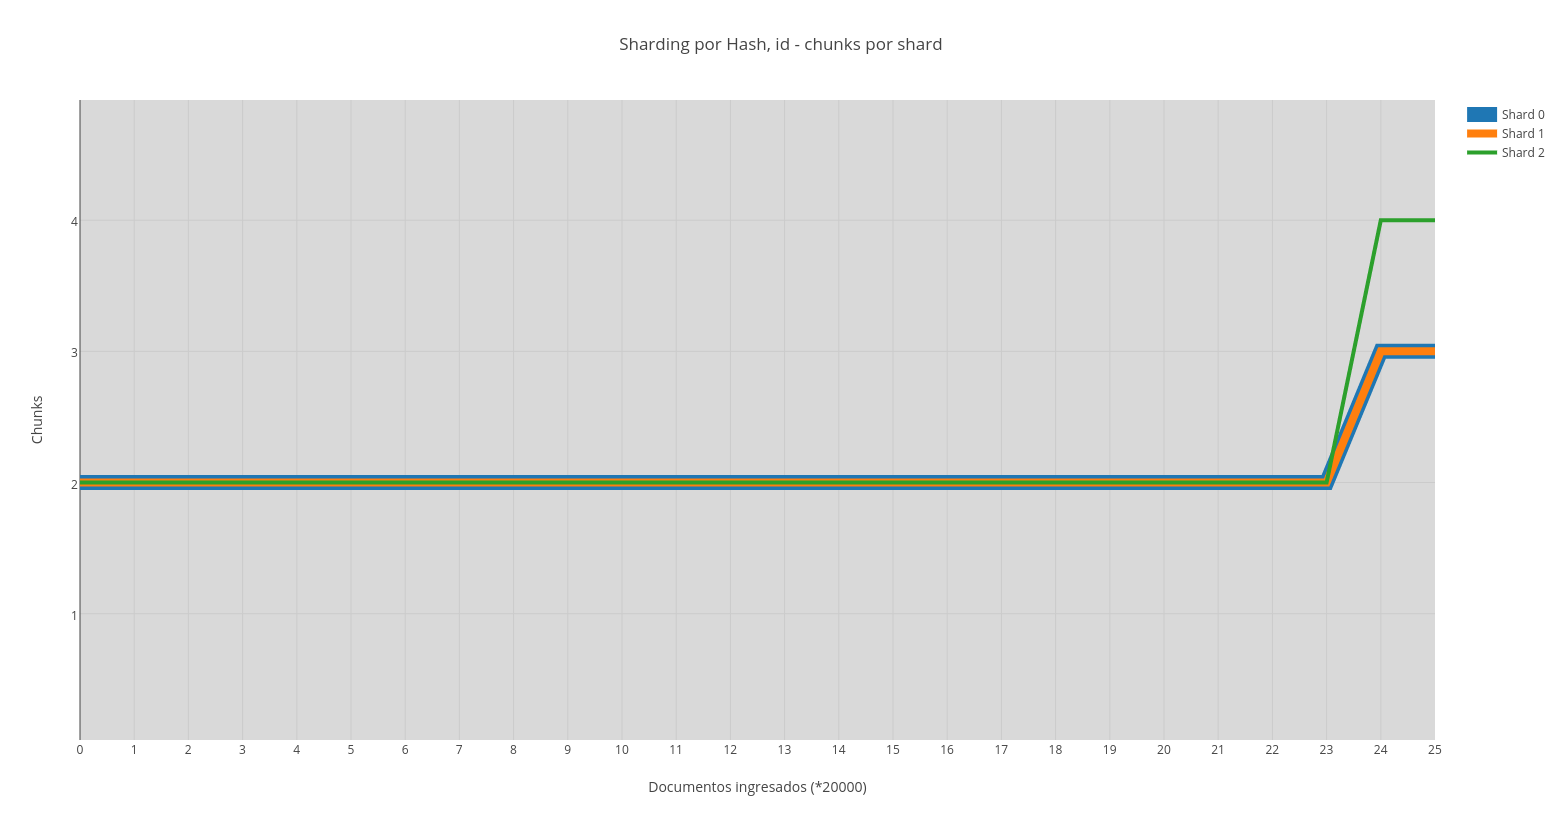
\includegraphics[scale=0.3]{./hash-cantidad-de-chunks-por-shard.png}
 \caption{Chunks por shard}
\end{figure}

Por último se muestra la cantidad de chunks por shard, permitiendo comparar mejor los gráficos anteriores.\\

Para observar mejor los gráficos se pueden acceder mediante los siguientes links a su representación online:
\begin{itemize}
 \item \href{https://plot.ly/~fzanollo/46/sharding-por-hash-id-documentos-por-shard/}{Documentos por shard}
 \item \href{https://plot.ly/~fzanollo/45/sharding-por-hash-id-documentos-estimados-por-chunk/}{Documentos estimados por chunk}
 \item \href{https://plot.ly/~fzanollo/44/sharding-por-hash-id-chunks-por-shard/}{Cantidad de chunks por shard}
\end{itemize}




\newpage
\subsection{Conclusión}

Es esencial elegir correctamente el shard key si se quiere una correcta distribución, hay que tener en cuenta distribución de los datos, cantidad de los mismos y cantidad de shards.\\

Hicimos el primer experimento (tipo de publicación) sin informarnos sobre cómo elegir el shard key, por suerte notamos los problemas a tiempo para repetir el experimento con otra key. Aunque respetando el enunciado no se eligió una shard key compuesta (índice simple). A vista de los resultados una posible clave sería la compuesta por (tipo de publicación, fecha) pero también depende de cómo se quiera acceder a los datos luego.\\

El índice hash funciona muy bien aunque se pierde la vecinidad de los datos, ya que datos con claves parecidas pueden ir a shards totalmente distintos. Esto puede ser algo tanto bueno como malo. Depende, nuevamente, de cómo se quieran utilizar los datos.

\subsection{Fuentes} 
\begin{itemize}
\item 
https://docs.mongodb.com/v3.0/sharding/
\item 
https://www.mongodb.com/blog/post/on-selecting-a-shard-key-for-mongodb
\item 
http://www.mongodbspain.com/es/tag/shard/
\end{itemize}
\newpage

\end{document}
